\documentclass[11pt,a4paper,oneside]{article}
\usepackage[utf8]{inputenc}
\usepackage[french]{babel}
\usepackage[T1]{fontenc}
\usepackage{graphicx}
\usepackage{charter}
\usepackage{hyperref}
\usepackage{listings}
\usepackage{wrapfig}

\usepackage[left=2cm,right=2cm,top=2cm,bottom=2cm]{geometry}
\usepackage{fancyhdr}
\pagestyle{fancy}
\usepackage{lastpage}
\renewcommand\headrulewidth{1pt}
\fancyhead[L]{Dossier Technique}
\renewcommand\footrulewidth{1pt}
\fancyfoot[C]{\textbf{Page \thepage/\pageref{LastPage}}}
\author{Mylann Dupuy}
\title{Dossier Technique --  \\ Powered by \LaTeX}
\date{5 Mars 2019 - Version 1.0}

\setlength{\parindent}{0cm}
\setlength{\parskip}{1ex plus 0.5ex minus 0.2ex}
\newcommand{\hsp}{\hspace{20pt}}
\newcommand{\HRule}{\rule{\linewidth}{0.5mm}}
\begin{document}

\begin{titlepage}
  \begin{sffamily}
  \begin{center}

    \textsc{\LARGE Dossier Technique - Powered by \LaTeX}\\[6.5cm]
    
\includegraphics[scale=1]{Ressources/polysoude.jpg}
    % Title
        \HRule \\[0.4cm]
        { \huge \bfseries TECHNICIEN SUPÉRIEUR DE SUPPORT INFORMATIQUE\\[0.4cm] }

        \HRule \\[6.5cm]

    % Author and supervisor
    \begin{minipage}{0.4\textwidth}
      \begin{flushleft} \large
        Candidat : Mylann \textsc{Dupuy}\\
        Promotion : HAPPT201\\
        Titre : T2SI
      \end{flushleft}
    \end{minipage}
    \begin{minipage}{0.5\textwidth}
      \begin{flushright} \large
        \emph{Tuteur :} M. Olivier \textsc{Naud}\\
        \emph{Binôme :} M. Antoine \textsc{Etrillard}\\
      \end{flushright}
    \end{minipage}

    \vfill

    % Bottom of the page
    {\large Version 2.0 - 05 Mars 2019}

  \end{center}
  \end{sffamily}
\end{titlepage}
\newpage
% ##### Page 2 #####
\tableofcontents
\newpage
\setcounter{page}{3}
\newpage

% ##### Page 3 #####
\section{Introduction}
Avant de parler de moi, je souhaiterais remercier l'entreprise qui m'a accueilli, il s'agit de \textbf{POLYSOUDE} ainsi qu'à l'équipe informatique qui me supporte depuis \textbf{Septembre 2017} au sein de leur service.

\subsection{Mon parcours}
Venant d'un \textbf{BAC PRO SEN} (Systèmes Électroniques Numériques) d'un lycée professionnel au Mans (72), j'ai poursuivi un \textbf{BTS SIO} que j'ai abandonné pour finalement être au sein de l'\textbf{ENI} depuis Septembre 2017 pour le titre \textbf{BAC +2 T2SI}

\subsection{Pourquoi cette formation et pas une autre ?}

C'est en recherchant une nouvelle formation que j'ai découvert l'existence du centre de formation de l'\textbf{ENI}.\\

En lisant les points qui allaient être étudier pendant la \textbf{formation T2SI} (qui m'était inconnue à ce jour), cela se rapprocher de ce que j'avais découvert pendant le BTS SIO mais sans les matières générales et qui m'a aussi permis d'en apprendre davantage. \\
\\
L'objectif que j'ai entrepris quand j'ai été accepté pour cette formation est de pouvoir décrocher le titre et ainsi intégrer une entreprise avec une possibilité d'évolution (dans le futur) avec un renouveau de mes connaissances et une ouverture d'esprit sur l'apprentissage et pour le travail en équipe.
\newpage

% ##### Page 4 #####
\section{Présentation de l'entreprise}
L'entreprise POLYSOUDE à été fondée en 1961 en se disant "pionnière dans la conception et la fabrication de matériel de soudage orbital". En 58 ans d'existence, l'entreprise à ouverte diverses filiales à travers le monde.\

Aujourd'hui, la maison mère de POLYSOUDE basée à Nantes compte 300 employés à son actif ainsi que 12 filiales / bureaux sans oublier les partenaires à travers le monde (+ de 50 partenaires). \\

\subsection{Hiérarchie}
L'organigramme ci-dessous résume en grande partie tous les différents départements que l'on peut y trouver actuellement.
\begin{figure}[h!]
  \centering
  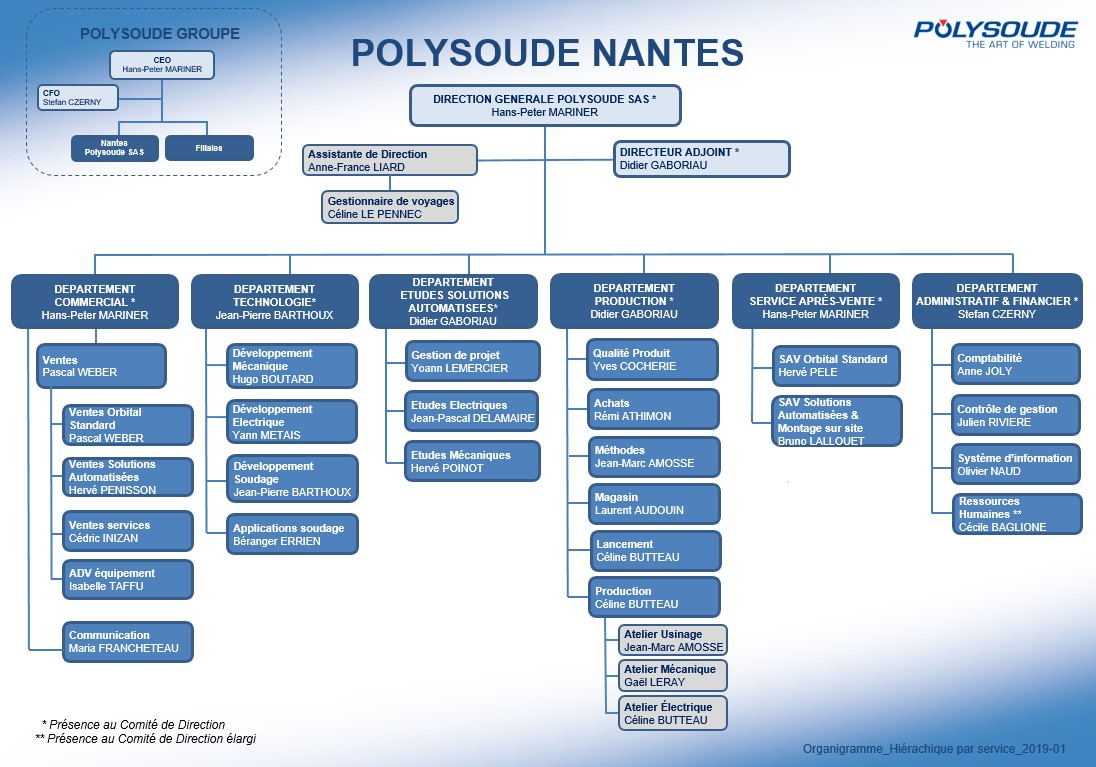
\includegraphics[width=\linewidth]{Ressources/Organigramme.jpg}
  \caption{Organigramme}
\end{figure}

Dans mon cas, mon collègue, \textbf{Antoine ETRILLARD} et moi-même somment dirigé par \textbf{Olivier NAUD} qui lui-même est dirigé par \textbf{Stefan CZERNY}.
\newpage

% ##### Page 5 #####
\section{Présentation de l'infrastructure}
L'infrastructure est gérée en interne, je m'explique :\

Les serveurs, qu'ils soient physique ou virtuels sont gérés par notre responsable et sous contrat chez différents prestataires / revendeurs.

Les utilisateurs utilisent tous une machine réelle que ce soit un poste fixe ou un poste portable.

Nos postes présents au sein des services sont présentés ci-dessous.\\
\newpage
% Schéma réseau
\rotatebox{90}{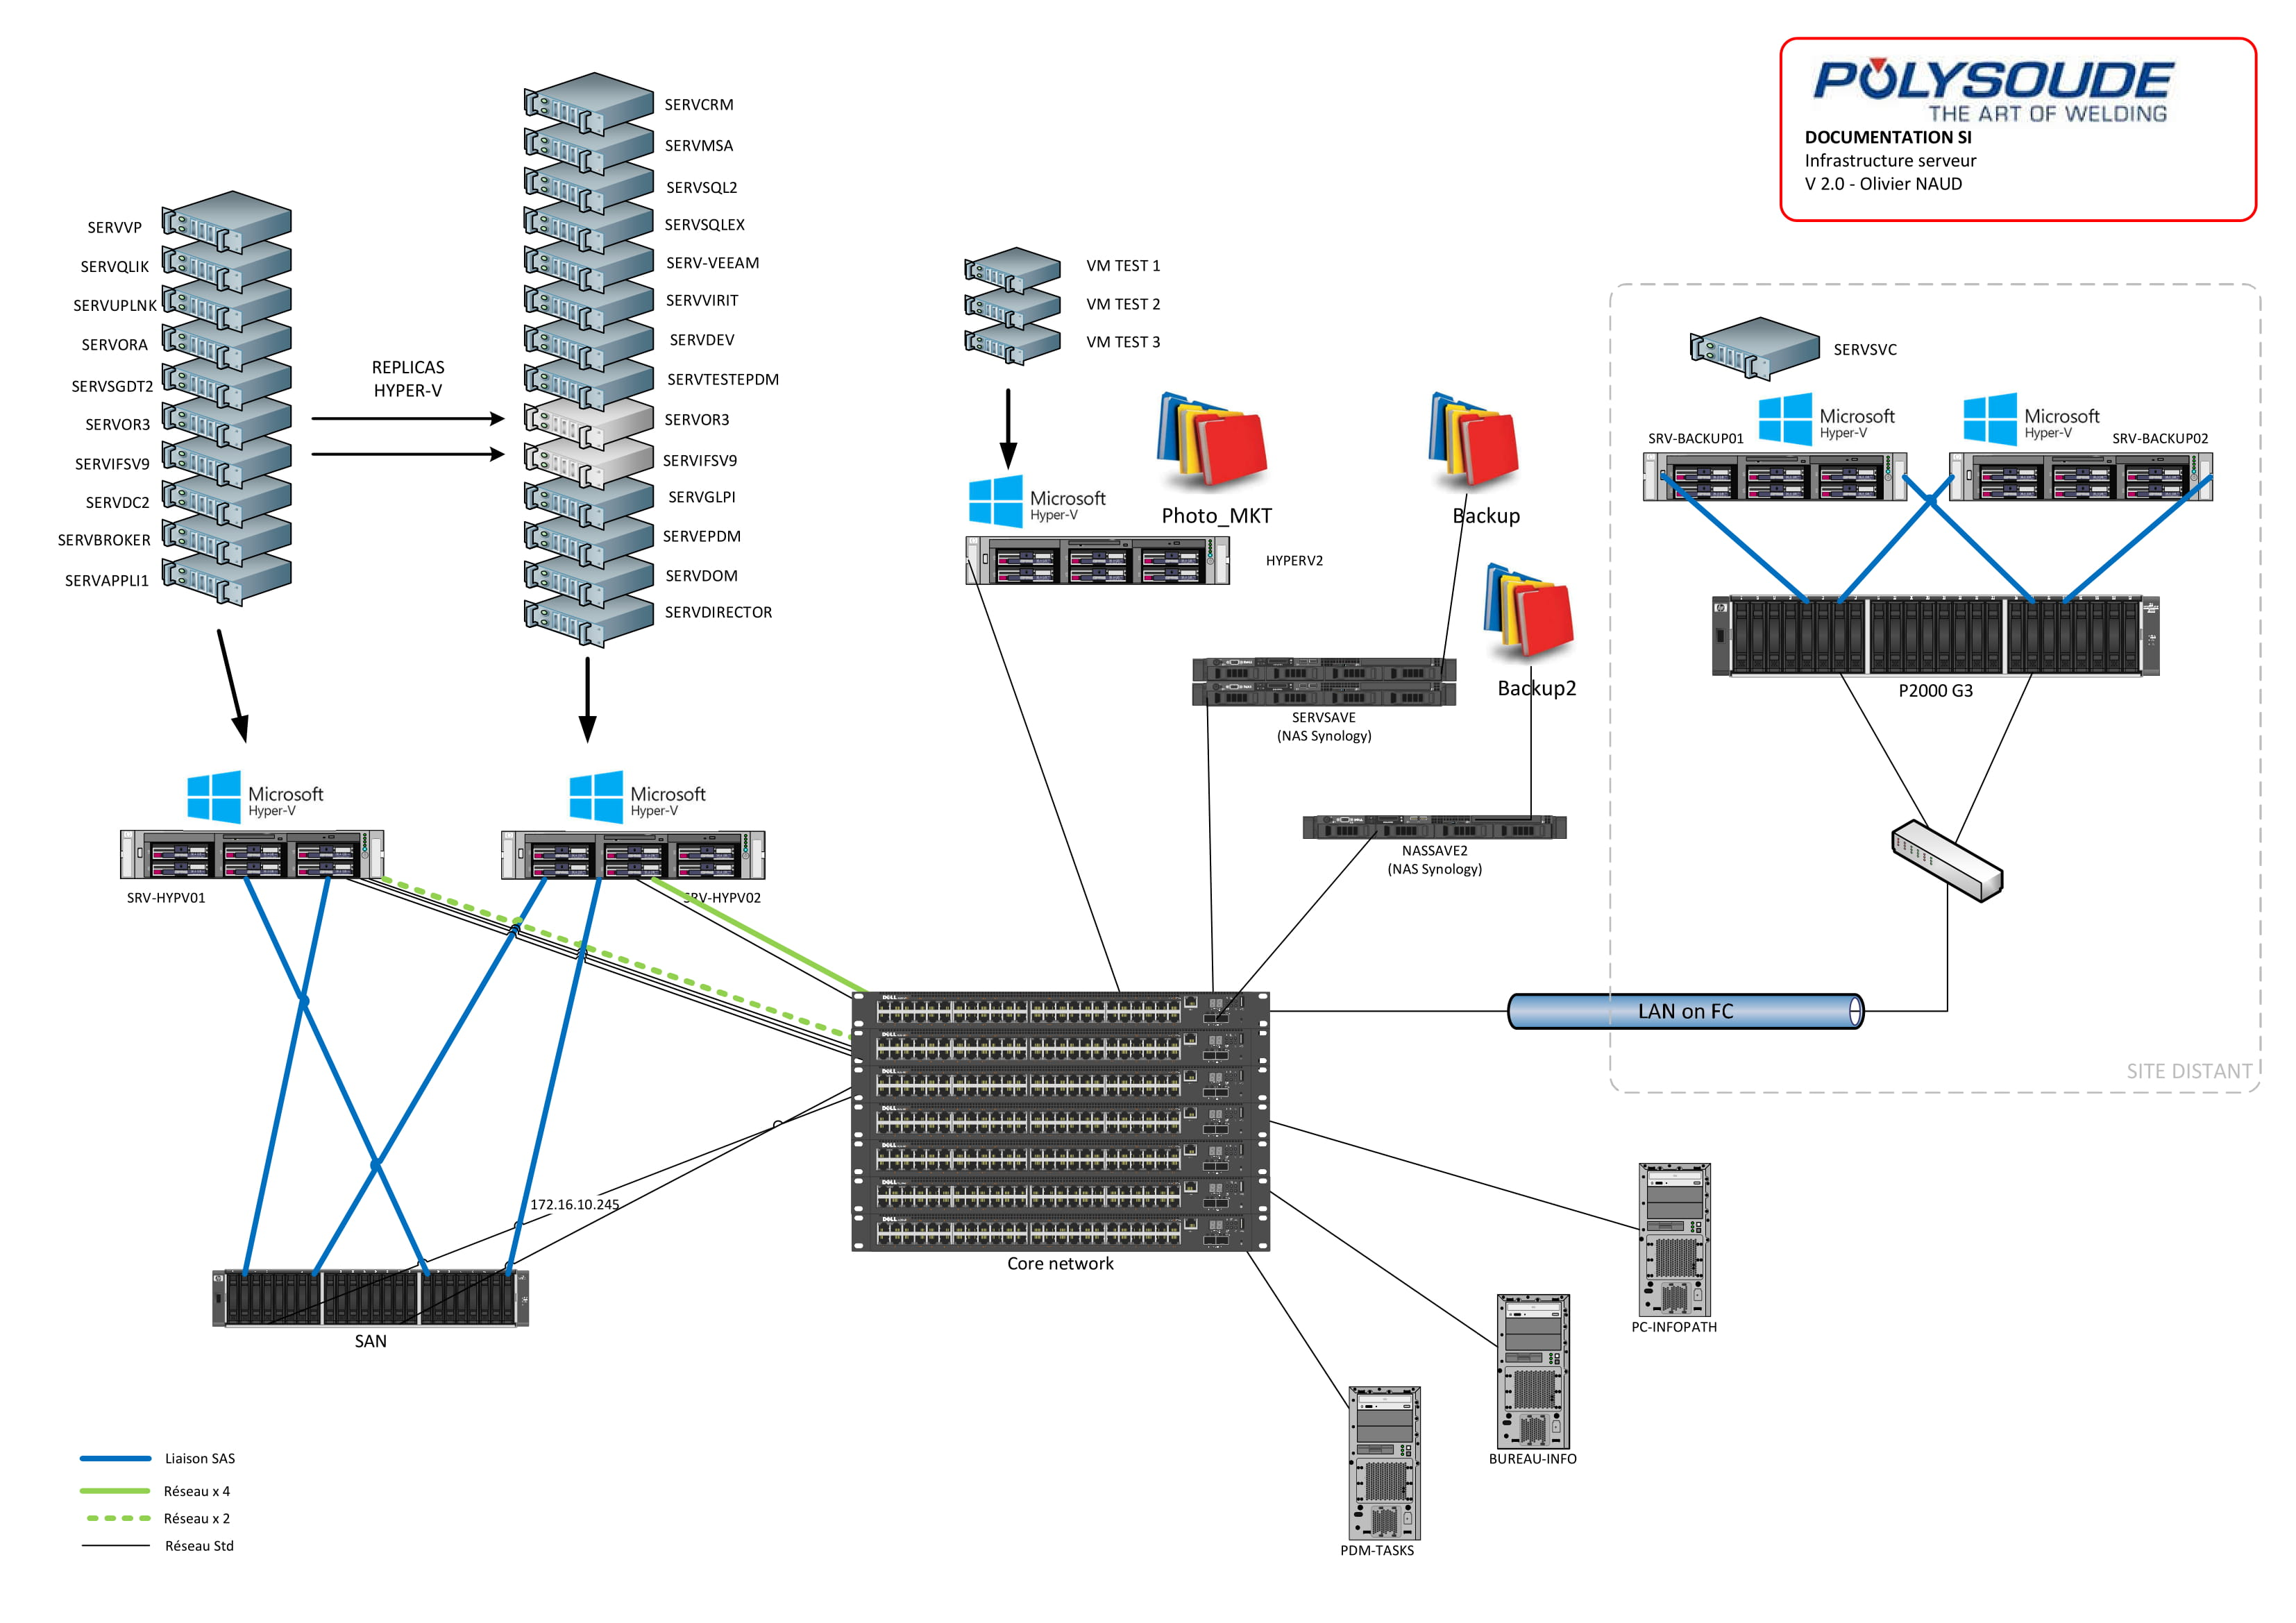
\includegraphics[scale=0.2]{Ressources/Reseau.jpg}}
\newpage
% Type matériel réel / Virtuel
\subsection{Parc Informatique}
\subsubsection{Postes Fixes}
% ### 1 ###
\begin{wrapfigure}{c}{7cm}
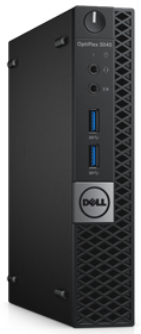
\includegraphics[scale=0.4]{Ressources/Materiel/3040.png}\vspace{-2cm}
\end{wrapfigure}
\paragraph{}\textbf{Dell OptiPlex 3040 Micro :} \\
\begin{itemize}
\item \textbf{CPU :} Intel Core i3
\item \textbf{RAM :} 8 Go
\item \textbf{OS :} Windows 7 / Windows 10
\item \textbf{Disque Dur :} 256 Go SDD / 500 Go HDD
\item \textbf{Quantité :} 41 unités
\\ \\ \\ \\
\end{itemize}
\begin{wrapfigure}{c}{7cm}
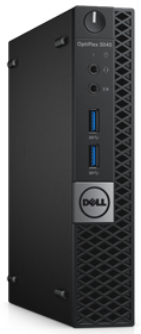
\includegraphics[scale=0.4]{Ressources/Materiel/3040.png}\vspace{-2cm}
\end{wrapfigure}
\paragraph{}\textbf{Dell Optiplex 3050 Micro :} \\
\begin{itemize}
\item \textbf{CPU :} A renseigner !!!
\item \textbf{RAM :} 8 Go
\item \textbf{OS :} Windows 7 / Windows 10
\item \textbf{Disque Dur :} 256 Go SSD // 500 Go HDD
\item \textbf{Quantité :} A renseigner !!!
\\ \\ \\ \\
\end{itemize}
\begin{wrapfigure}{c}{7cm}
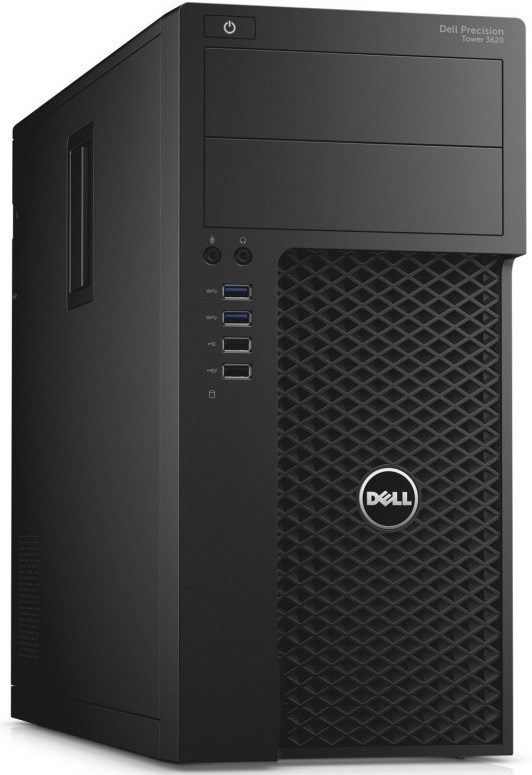
\includegraphics[scale=0.3]{Ressources/Materiel/3620.jpg}\vspace{-2cm}
\end{wrapfigure}
\paragraph{}\textbf{Dell Precision 3620 :} \\
\begin{itemize}
\item \textbf{CPU :} A renseigner !!!
\item \textbf{RAM :} 8 Go
\item \textbf{OS :} Windows 7
\item \textbf{Disque Dur :} 256 Go SSD // 500 Go SSHD
\item \textbf{Quantité :} A renseigner !!!
\\ \\ \\ \\
\end{itemize}

\newpage
\subsubsection{Postes Portables}
% ### 2 ###
\begin{wrapfigure}{c}{7cm}
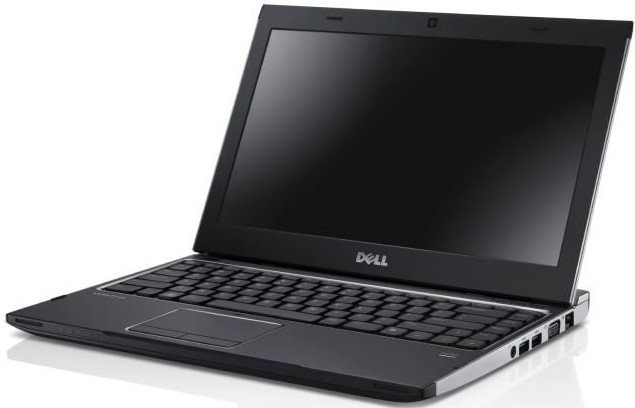
\includegraphics[scale=0.4]{Ressources/Materiel/V131.jpg}\vspace{-2cm}
\end{wrapfigure}
\paragraph{}\textbf{Dell Vostro V131 :} \\
\begin{itemize}
\item \textbf{CPU :} Intel Core i5-2410M
\item \textbf{RAM :} 8 Go
\item \textbf{OS :} Windows 7
\item \textbf{Disque Dur :} 500 Go HDD
\item \textbf{Quantité :} 13 unités
\\ \\ \\ \\
\end{itemize} 
% ### 3 ###
\begin{wrapfigure}{c}{7cm}
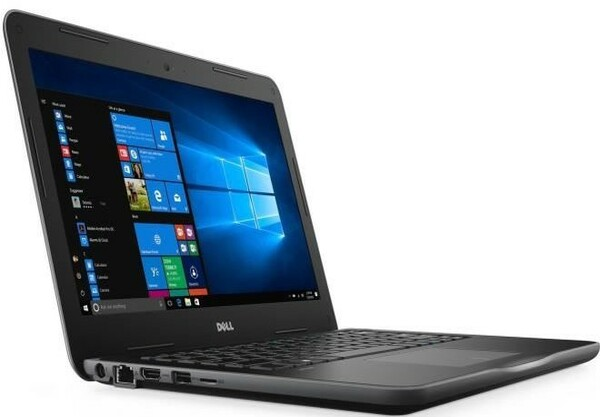
\includegraphics[scale=0.4]{Ressources/Materiel/L3380.jpg}\vspace{-2cm}
\end{wrapfigure}
\paragraph{}\textbf{Dell Latitude 3380 :} \\
\begin{itemize}
\item \textbf{CPU :} Intel Core i5-7200U
\item \textbf{RAM :} 8 Go
\item \textbf{OS :} Windows 7
\item \textbf{Disque Dur :} 256 Go SSD / 500 Go HDD
\item \textbf{Quantité :} 17 unités
\\ \\ \\ \\
\end{itemize}
\newpage
% ### 4 ###
\begin{wrapfigure}{c}{7cm}
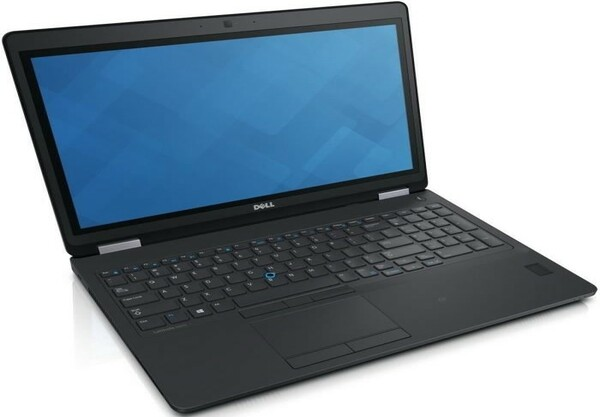
\includegraphics[scale=0.4]{Ressources/Materiel/LE5570.jpg}\vspace{-2cm}
\end{wrapfigure}
\paragraph{}\textbf{Dell Latitude E5570 :} \\
\begin{itemize}
\item \textbf{CPU :} Intel Core i7-6820HQ
\item \textbf{RAM :} 8 Go
\item \textbf{OS :} Windows 10
\item \textbf{Disque Dur :} 256 Go SSD
\item \textbf{Quantité :} 4 unités
\\ \\ \\ \\
\end{itemize}
% ### 5 ###
\begin{wrapfigure}{c}{7cm}
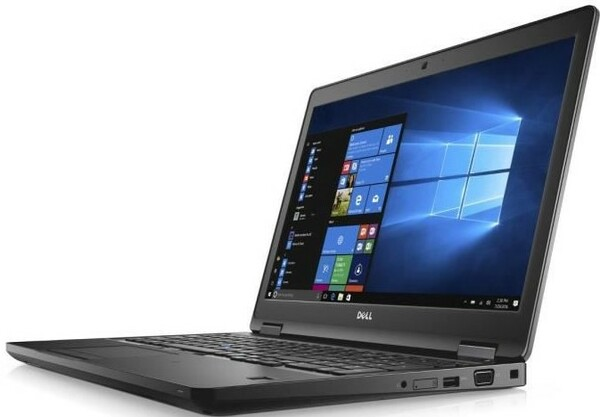
\includegraphics[scale=0.4]{Ressources/Materiel/L5580.jpg}\vspace{-2cm}
\end{wrapfigure}
\paragraph{}\textbf{Dell Latitude 5580 :} \\
\begin{itemize}
\item \textbf{CPU :} Intel Core i7-6820HQ
\item \textbf{RAM :} 8 Go
\item \textbf{OS :} Windows 10
\item \textbf{Disque Dur :} 256 Go SSD
\item \textbf{Quantité :} 5 unités
\\ \\ \\ \\ \\
\end{itemize}
% ### 6 ###
\begin{wrapfigure}{c}{7cm}
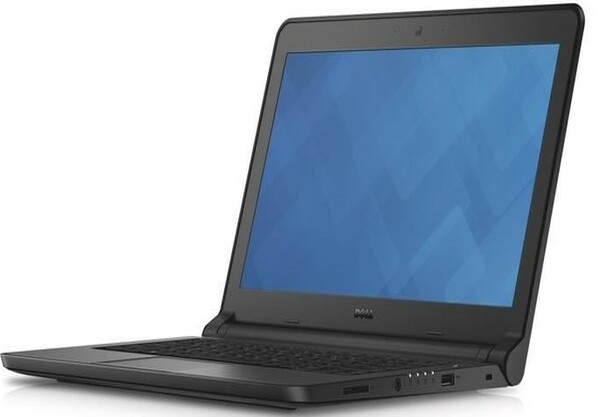
\includegraphics[scale=0.4]{Ressources/Materiel/L3340.jpg}\vspace{-2cm}
\end{wrapfigure}
\paragraph{}\textbf{Dell Latitude 3340 :} \\
\begin{itemize}
\item \textbf{CPU :} Intel Core i5-4210U
\item \textbf{RAM :} 8 Go
\item \textbf{OS :} Windows 10
\item \textbf{Disque Dur :} 256 Go SSD
\item \textbf{Quantité :} 23 unités
\\ \\ \\ \\
\end{itemize}
% ### 7 ###
\begin{wrapfigure}{c}{7cm}
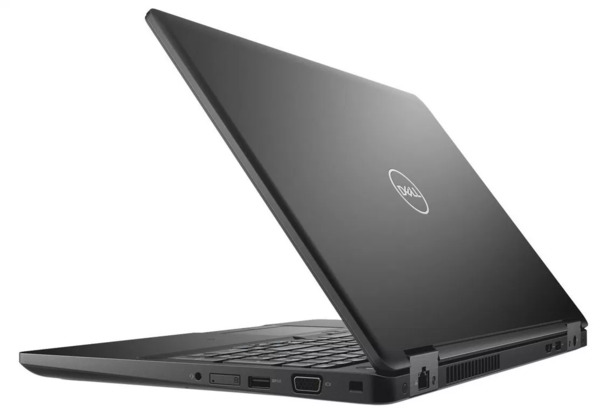
\includegraphics[scale=0.35]{Ressources/Materiel/L5591.jpg}\vspace{-2cm}
\end{wrapfigure}
\paragraph{}\textbf{Dell Latitude 5591 :} \\
\begin{itemize}
\item \textbf{CPU :} Intel Core i5-4210U
\item \textbf{RAM :} 8 Go
\item \textbf{OS :} Windows 10
\item \textbf{Disque Dur :} 256 Go SSD
\item \textbf{Quantité :} 14 unités
\\ \\ \\ \\
\end{itemize}
% ### 8 ###
\begin{wrapfigure}{c}{7cm}
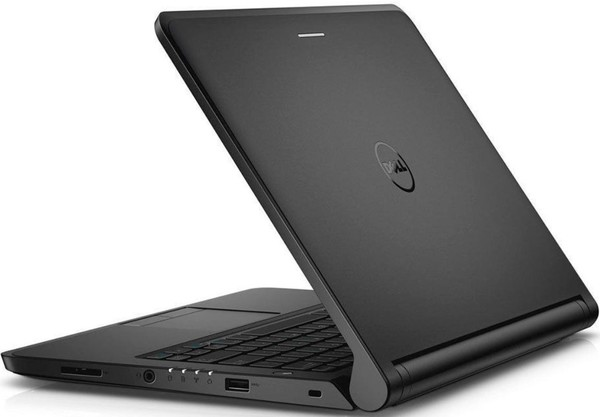
\includegraphics[scale=0.4]{Ressources/Materiel/L3350.jpg}\vspace{-2cm}
\end{wrapfigure}
\paragraph{}\textbf{Dell Latitude 3350 :} \\
\begin{itemize}
\item \textbf{CPU :} Intel Core i5-4210U
\item \textbf{RAM :} 8 Go
\item \textbf{OS :} Windows 10
\item \textbf{Disque Dur :} 256 Go SSD
\item \textbf{Quantité :} 14 unités
\\ \\ \\ \\
\end{itemize}
% ### 7 ###
\newpage
\subsection{Serveurs}
\subsubsection{Physiques}
bla bla
\subsubsection{Virtuels}
bla bla
% Activités
\newpage

% ##### Page 6 #####
\section{Objectif(s) du stage}

Lors de l'entretien d'embauche, le responsable informatique voulait une personne autonome, vif et capable d'agir (en fonction de la demande) et travailler en équipe.
\\ \\
Pour moi, c'était la 1\ier fois que j'avais ce genre de mission et de responsabilité au sein d'un parc de plus de 150 postes et surtout avec une équipe.
\\ \\
Les tâches qui m'ont été confiées au fil du temps étaient : 
\begin{itemize}
    \item Répondre aux appels téléphonique pour une intervention par téléphone.
    \item Assurer la gestion de parc.
    \item Former les utilisateurs sur les outils / matériels mis à disposition.
    \item Utiliser l'outil de ticketing GLPI.
    \item Réinitialiser les mots de passe des utilisateurs.
    \item Déploiement de poste.
    \item Gestion des demandes matériels.
    \item Ouvrir des tickets de support chez nos différents prestataire.
\end{itemize}
\newpage

% ##### Page 7 ######
\section{Environnement du stage}
\newpage

% ##### Page 8 ######
\section{Présentation des principales activités \& réalisation durant le stage}
\subsection{Support utilisateur}

\begin{figure}[!h]
\centering
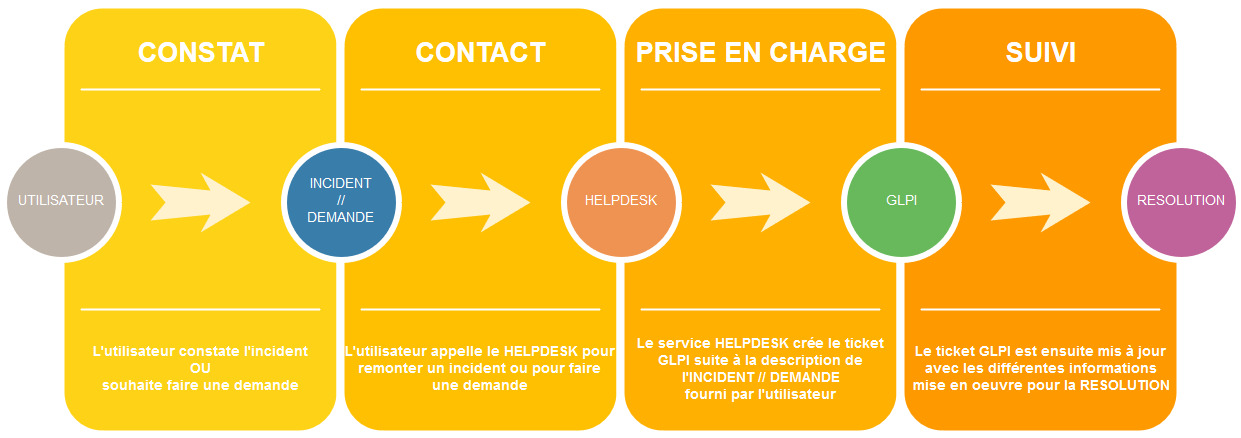
\includegraphics[scale=0.42]{Ressources/GLPI.jpg}
\caption{\label{Schéma de support}}
\end{figure}
\newpage

% ##### Page 9 ######
\subsection{Déploiement de poste}
\newpage

% ##### Page 10 ######
\subsection{Administration}
\newpage

\end{document}